\chapter{Lesson Plans} \label{chap:lessonplan}
With the addition of a JSON printer capable of generating Jupyter Notebooks, we 
are now looking to expand Drasil's application by generating educational 
documents. As discussed in Chapter~\ref{chap:intro}, Jupyter Notebooks are 
commonly used in teaching engineering courses due to their characteristics and 
advantages. One of the educational practices to enhance teaching is creating 
lesson plans \cite{cicek2013effective, wong2018first}, which provide a 
guide for structuring daily activities in each class period. A lesson plan 
outlines the learning objectives, methods and procedures for achieving them, 
and metrics for student progress. Lesson plans are an ideal starting 
point for generating educational documents in Drasil because they are more 
accessible than academic papers. In addition, we are able to work with real 
examples in a lesson plan. 

To incorporate lesson plans in Drasil, we first need to understand their 
components and categorize the knowledge in a structured manner. We analyzed the 
similarities and differences of elements in textbook chapters in 
\href{https://github.com/smiths/caseStudies/blob/master/CaseStudies/projectile/projectileLesson/AboutProjectileLesson.pdf}{Discussion
 of Projectile Lesson: What and	Why} using online resources. Based on our 
analysis, we narrowed down the elements and defined a structure that fits our 
lesson plans the most, as summarized in Table~\ref{tab:lessonPlanstrucutre}. 
While not all chapters are mandatory, a typical lesson plan includes learning 
outcomes (objectives), lesson topics (case problems), and activities (examples).
It's worth noting that this structure may be subject to future modifications to 
better suit our needs. 

\begin{longtable}[c]{|>{\raggedright}p{0.25\linewidth}|>{\raggedright\arraybackslash}p{0.7\linewidth}|}
	\caption{Structure of Lesson Plans} 
	\label{tab:lessonPlanstrucutre}                                            
	\\ \hline
	
	\rowcolor{McMasterMediumGrey}
	\textbf{Chapter} & \textbf{Overview}
	\\ \hline
	
	Introduction & An introduction of the lesson plan or the topic.
	\\ \hline
	Learning Objectives & What students can do or will learn after the 
	lesson.  
	\\ \hline
	Review & A recap of what has been covered previously.
	\\ \hline
	A Case Problem & A case problem that link the topic to a real world 
	problem.
	\\ \hline
	Example & An example of the case problem.
	\\ \hline
	Summary & A summary of the lesson plan.
	\\ \hline
	Bibliography & References that support the lesson plan.
	\\ \hline
	Appendix & Additional resources or information of the lesson.
	\\ \hline
\end{longtable}

In this chapter, we will discuss the language of lesson plans in Drasil, 
introduce a new case study on Projectile Motion Lesson, and explore the reuse 
of knowledge in Drasil.

\section{Language of Lesson Plans} \label{chap:lessonLang}
To generate a new type of document, lesson plans, in Drasil, we must define its 
language first. Drasil's document language has SRS, and we are creating a 
language for lesson plans. As discussed in Chapter~\ref{chap:nbprinter}, a 
Drasil document has a title, authors, and sections, which hold the contents 
of the document. The definition of a document is defined in 
\textbf{drasil-lang}\footnote{\textbf{drasil-lang} holds the higher level 
language for Drasil.} as shown in 
Code~\ref{code:drasil-lang-document}\footnote{\texttt{ShowToC} is 
\texttt{ShowTableOfContents} in the source code, which is to determine whether 
to show the table of contents in the document.}, where \texttt{Document} is the 
type for SRS document and \texttt{Notebook} is for Jupyter Notebook, 
specifically lesson plans at this moment. The reason why we define them 
separately is because we print the SRS and lesson plans differently. We are 
able to pattern match the way we print the document in the printer.

\begin{listing}[h]
	\caption{Code for Definition of Document}
	\label{code:drasil-lang-document}
	\begin{lstlisting}[language=haskell1]
		data Document = Document Title Author ShowToC [Section]
									| Notebook Title Author [Section]
	\end{lstlisting}
\end{listing}

We need to create helper types and functions that facilitate the creation of 
document language for generating lesson plans, based on our lesson plans 
structure. Our first step is to define the types and data for the lesson and 
its chapters in Drasil's document language, \textbf{drasil-docLang}. 
Code~\ref{code:core} is the core declaration of the lesson plan. A 
\texttt{LsnDesc} type represents a lesson description (line 1), which consists 
of lesson chapters (line 3), including an introduction, learning objectives, 
review, case problem, example, summary, bibliography, and appendix. The detail 
structure of each chapter is defined in line 12-31. At present, 
\texttt{Contents} is the only defined elements as the chapter structure has not 
yet been fully understood. We intend to further develop the chapter structure 
in the future.

\begin{listing}[h!]
	\caption{Source Code for Notebook Core Language}
	\label{code:core}
	\begin{lstlisting}[language=haskell1]		
		type LsnDesc = [LsnChapter]

		data LsnChapter = Intro Intro
										| LearnObj LearnObj
										| Review Review
										| CaseProb CaseProb
										| Example Example
										| Smmry Smmry
										| BibSec
										| Apndx Apndx
		
		-- ** Introduction
		newtype Intro = IntrodProg [Contents]		
		-- ** Learning Objectives
		newtype LearnObj = LrnObjProg [Contents]		
		-- ** Review Chapter
		newtype Review = ReviewProg [Contents]		
		-- ** A Case Problem
		newtype CaseProb = CaseProbProg [Contents]		
		-- ** Examples of the lesson
		newtype Example = ExampleProg [Contents]		
		-- ** Summary
		newtype Smmry = SmmryProg [Contents]		
		-- ** Appendix
		newtype Apndx = ApndxProg [Contents]
	\end{lstlisting}
\end{listing}

The \texttt{LsnDecl} type, as shown in Code~\ref{code:LsnDecl}, is used to 
declare all the necessary chapters for a lesson plan. It is similar in 
definition to \texttt{LsnDesc}, but in a more usable form. It is meant to be a 
semantic rendition of a lesson plan document, while \texttt{LsnDesc} is 
intended to be a general description and more suitable for printing 
\cite{lsnDeclandlsnDesc}. They are identical at this point because the chapter 
structure is not well understood, but they might evolve differently as we gain 
more understanding of our lesson plans.

\begin{listing}[h]
	\caption{Source Code for LsnDecl}
	\label{code:LsnDecl}
	\begin{lstlisting}[language=haskell1]
		type LsnDecl  = [LsnChapter]
		
		data LsnChapter = Intro NB.Intro
										| LearnObj NB.LearnObj
										| Review NB.Review
										| CaseProb NB.CaseProb
										| Example NB.Example
										| Smmry NB.Smmry
										| BibSec
										| Apndx NB.Apndx
	\end{lstlisting}
\end{listing}

\begin{listing}[h!]
	\caption{Source Code for Section and the section Constructor}
	\label{code:section}
	\begin{lstlisting}[language=haskell1]
		data Section = Section
								  { tle  :: Title
								  , cons :: [SecCons]
								  , _lab :: Reference
								  }
		makeLenses ''Section
		
		-- | Constructor for creating 'Section's with a title 
		-- ('Sentence'), introductory contents, a list of 
		-- subsections, and a	shortname ('Reference').
		section :: Sentence -> [Contents] -> [Section] -> Reference -> Section
		section title intro secs = Section title (map Con intro ++ map Sub secs)
	\end{lstlisting}
\end{listing}

Next, we need functions to generate chapters. We can use the \texttt{Section} 
type that is used for creating SRS sections, which consists of a title, a list 
of contents, and a short name, as shown in Code~\ref{code:section}. We can also 
take advantage of the \texttt{section} smart constructor to build our own 
chapter constructors, as illustrates in Code~\ref{code:chapterConstructor}. 
Once we have these constructors, we can use them to build each chapter 
(Code~\ref{code:mkChapters}).

\begin{listing}[h!]
	\caption{Source Code for Chapter Constructors} 
	\label{code:chapterConstructor}
	\begin{lstlisting}[language=haskell1]
		learnObj, review, caseProb, example :: [Contents] -> 
				[Section] -> Section
		learnObj cs ss = section (titleize' Docum.learnObj) cs ss learnObjLabel
		review   cs ss = section (titleize Docum.review)    cs ss reviewLabel
		caseProb cs ss = section (titleize Docum.caseProb)  cs ss caseProbLabel
		example  cs ss = section (titleize Docum.example)   cs ss exampleLabel
	\end{lstlisting}
\end{listing}

\begin{listing}[h!]
	\caption{Source Code for Making Chapters} 
	\label{code:mkChapters}
	\begin{lstlisting}[language=haskell1]				
		-- | Helper for making the 'Learning Objectives'.
		mkLearnObj :: LearnObj -> Section
		mkLearnObj (LrnObjProg cs) = Lsn.learnObj cs []
		
		-- | Helper for making the 'Review'.
		mkReview :: Review -> Section
		mkReview (ReviewProg r) = Lsn.review r [] 
		
		-- | Helper for making the 'Case Problem'.
		mkCaseProb :: CaseProb -> Section
		mkCaseProb (CaseProbProg cp) = Lsn.caseProb cp [] 
		
		-- | Helper for making the 'Example'.
		mkExample:: Example -> Section
		mkExample (ExampleProg cs) = Lsn.example cs []
	\end{lstlisting}
\end{listing}

When building lesson plans, the document and chapters are encoded in the 
\texttt{LsnDecl} type, which is then converted to \texttt{LsnDesc} for 
printing. The \texttt{mkNb} function, as shown in Code~\ref{code:mkNb}, takes 
the user-encoded list of chapters (i.e., \texttt{LsnDecl}) and \texttt{System 
Information}\footnote{System Information is a data structure designed to 
contain all the necessary information about a system for the purpose of 
generating artifacts.} to form a lesson plan document. The \texttt{mkSections} 
and \texttt{mkLsnDesc} functions are helper functions that aid in the creation 
of lesson plan chapters.

\begin{listing}[h!]
	\caption{Source Code for mkNb}
	\label{code:mkNb}
	\begin{lstlisting}[language=haskell1]
		mkNb :: LsnDecl -> (IdeaDict -> IdeaDict -> Sentence) 
			 -> SystemInformation -> Document
		mkNb dd comb si@SI {_sys = s, _kind = k, _authors = a} =
			Notebook (nw k `comb` nw s) (foldlList Comma List $ 
				map (S . name) a) $	mkSections si l where
					l = mkLsnDesc si dd
	\end{lstlisting}
\end{listing}

All types and functions discussed in this chapter are declared in 
\textbf{drasil-docLang}. Table~\ref{tab:notebookLang} provides an overview of 
the responsibilities of each module regarding the language of lesson plans. 
Complete implementation of the language of lesson plans can be found in 
Code~\ref{code:docLang_notebook} to Code~\ref{code:notebook_LsnDecl} in 
Appendix A.

\begin{longtable}[c]{|>{\raggedright}p{0.27\linewidth}|>{\raggedright\arraybackslash}p{0.69\linewidth}|}
	\caption{Summary of Notebook Modules} 
	\label{tab:notebookLang}                                              
	\\ \hline
	
	\rowcolor{McMasterMediumGrey}
	\textbf{Module} & \textbf{Responsibility}
	\\ \hline
	\multicolumn{2}{|l|}{\textbf{Drasil.DocLang}} 
	\\ \hline
	Notebook.hs & Contains constructors for building chapters.
	\\ \hline
	\multicolumn{2}{|l|}{\textbf{Drasil.DocumentLanguage.Notebook}} 
	\\ \hline
	Core.hs & Contains general description functions for lesson plans.
	\\ \hline
	DocumentLanguage.hs & Holds functions to create chapters and form a lesson 
	plan.
	\\ \hline
	LsnDecl.hs & Contains declaration functions for generating lesson plans. 
	\\ \hline
\end{longtable}


\section{A Case Study: Projectile Motion} \label{chap:projMotion}
In Chapter~\ref{chap:lessonLang}, we discussed the language of lesson plans to 
introduce a new case study on projectile motion. We chose projectile motion as 
a starting point for our lesson plans for several reasons: i) it is often one 
of the initial concepts taught when students are introduced to the study of 
dynamics; ii) the developed model is considered relatively straightforward as 
it solely incorporates kinematics, which pertains to the geometric 
characteristics of motion \cite{smith2022projectile}; iii) Drasil already 
captures the knowledge of projectile, allowing us to showcase the reuse of 
knowledge. We are going to reproduce the 
\href{https://github.com/smiths/caseStudies/blob/master/CaseStudies/projectile/projectileLesson/orgModeVersion/projMotLesson.pdf}{Projectile
 Motion Lesson}, authored by Dr. Spencer Smith, and generate a Jupyter Notebook 
 version with Drasil.

In accordance with the lesson plan structure discussed, we divided the 
\href{https://github.com/smiths/caseStudies/blob/master/CaseStudies/projectile/projectileLesson/orgModeVersion/projMotLesson.pdf}{Projectile
 Motion Lesson} into four chapters: learning objectives, review, a case 
problem, and examples. Each chapter is composed of a variety of content types, 
such as sentences, equations, or figures. To combine these contents into a 
chapter, we convert them to the \texttt{Contents} type and map them together. 
We provide smart constructors like \texttt{lbldExpr}\footnote{This converts a 
\texttt{ModelExpr} into a \texttt{Contents}.} for transfering different kind of 
contents to \texttt{Contents}. In Code~\ref{code:reviewContent}, we demonstrate 
how information and contents of the review chapter are encoded in Drasil.

\begin{listing}[h!]
	\caption{Source Code for Encoded Review Chapter} 
	\label{code:reviewContent}
	\begin{lstlisting}[language=haskell1]	
		reviewContent :: [Contents]
		reviewContent = [reviewHead, reviewContextP1, 
			LlC E.lcrectVel, LlC E.lcrectPos, LlC E.lcrectNoTime, 
			reviewEqns, reviewContextP2]
		
		reviewHead, reviewContextP1, 
			reviewEqns, reviewContextP2 :: Contents
		reviewHead = foldlSP_ [headSent 2 (S "Rectilinear 
			Kinematics: Continuous Motion")]
		reviewContP1 = foldlSP_
			[S "As covered previously, the", plural equation, S 
	 		 "relating", phrase velocity, sParen (eS (sy QP.speed)
	 		 ) `sC` phrase position, sParen (eS (sy QP.scalarPos)) 
	 		 `S.and_` phrase time, sParen (eS (sy QP.time)) 
	 		 `S.for` phrase motion `S.in_` S "one dimension with",
	 		 phrase QP.constAccel, sParen (eS (sy QP.constAccel)) 
	 		 +:+ S "are as follows:"]
		
		reviewEqns = foldlSP [S "where", eS (sy QP.iSpeed) 
			`S.and_` eS (sy QP.iPos), S "are the initial",
			 phrase velocity `S.and_` phrase position, 
			 S ",respectively"]
		
		reviewContP2 = foldlSP 
			[S "Only two of these", plural equation, S "are 
	 		 independent, since the third" +:+ phrase equation, S 
	 		 "can always be derived from the other two"]
	\end{lstlisting}
\end{listing}

A lesson plan is represented in the \texttt{LsnDecl} type, which is a 
collection of chapters (see Code~\ref{code:mkNB}). We then use the 
\texttt{mkNb} function (presented in Code~\ref{code:mkNb}) to convert the 
lesson plan into a Drasil document. The resulting document can be printed and 
produced as a Jupyter Notebook with the Drasil printer, as discussed in 
Chapter~\ref{chap:nbprinter}.

\begin{listing}[h!]
	\caption{Source Code for Forming a Notebook} 
	\label{code:mkNB}
	\begin{lstlisting}[language=haskell1]				
		mkNB :: LsnDecl
		mkNB = [
			LearnObj $ LrnObjProg [learnObjContext],
			Review $ ReviewProg reviewContent,
			CaseProb $ CaseProbProg caseProbCont,
			Example $ ExampleProg exampleContent,
			BibSec
		]
	\end{lstlisting}
\end{listing}

The review chapter of Projectile Motion Lesson created manually and using 
Drasil can be seen in Figures~\ref{fig:review_manual} and 
\ref{fig:review_drasil}, respectively. Moreover, Figure~\ref{fig:review_drasil} 
is generated from the code presented in Code~\ref{code:reviewContent}.

\begin{figure}[h!]
	\caption{Review Chapter Created Manually}
	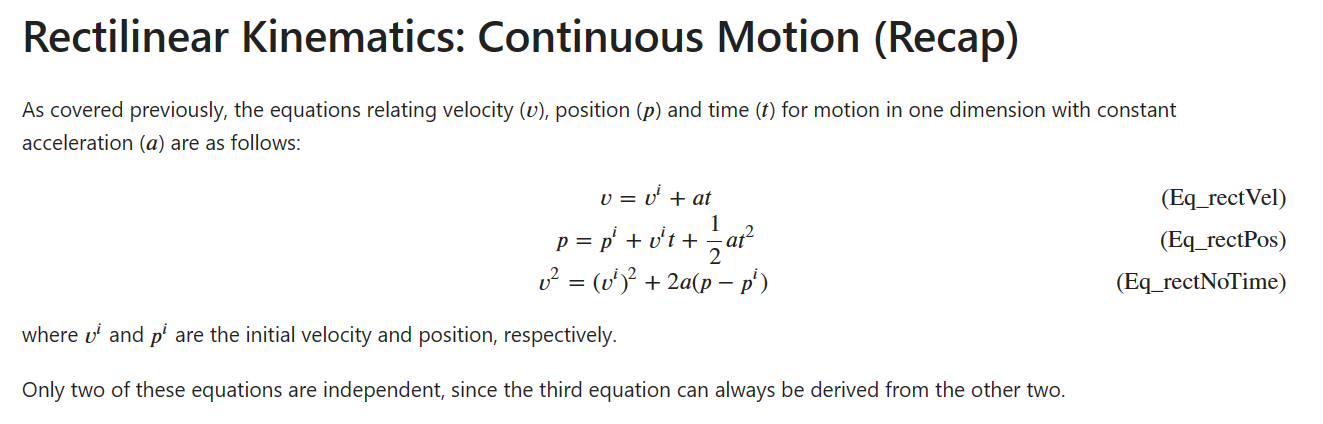
\includegraphics[width=1\textwidth]{figures/review_manual.png}
	\label{fig:review_manual}
\end{figure}

\begin{figure}[h!]
	\caption{Review Chapter Generated using Drasil}
	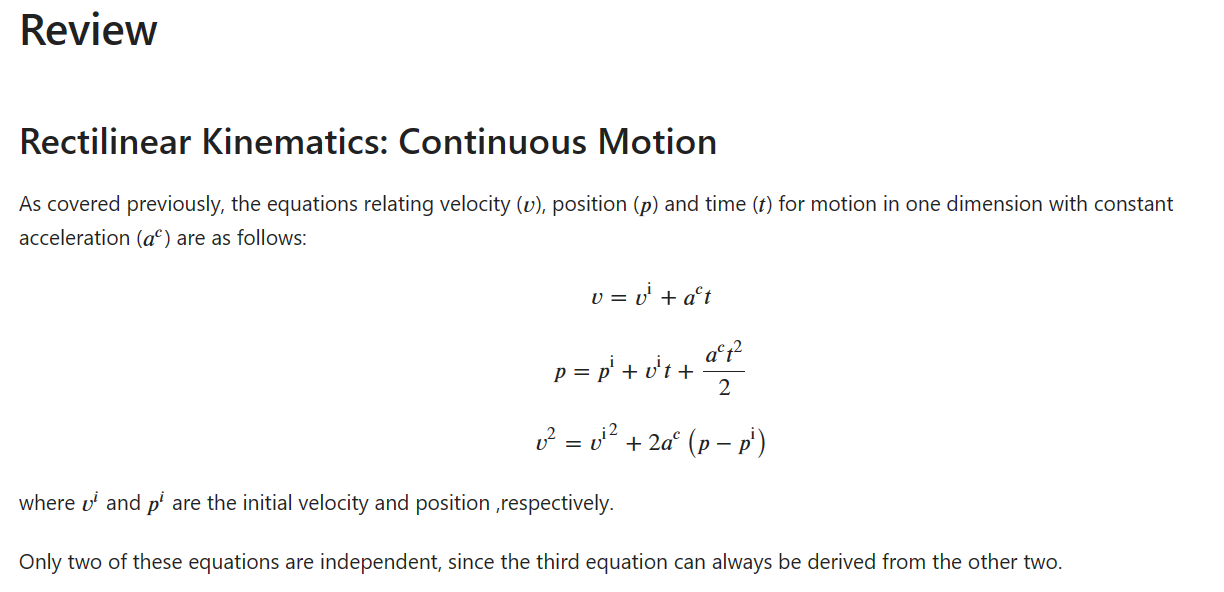
\includegraphics[width=1\textwidth]{figures/review_drasil.png}
	\label{fig:review_drasil}
\end{figure}

The remaining chapters of the generated Projectile Motion Lesson can be found 
in Appendix A, from Figure~\ref{fig:learnObj} to Figure~\ref{fig:caseProb-5}. 

\section{Knowledge Reusability}
Drasil offers the advantage of reusing knowledge, which is not trivial. We 
would like to highlight this feature with the Projectile and Projectile Motion 
Lesson. 

In Drasil, we store commonly used knowledge, such as physics concepts (e.g., 
acceleration) and mathematics ideas (e.g., Cartesian coordinates), in a package 
named \textbf{drasil-data}. Additionally, each case study has its own package 
that contains concepts specific to that study. For example, ``Projectile 
Motion" is an idea in the Projectile case study. Once these ideas and concepts 
are defined in Drasil, they can be utilized whenever needed. Since there is an 
overlap in knowledge between the Projectile SRS and Projectile Motion Lesson, 
we can reuse the information without the need to encode it again.

For example, the following equation is the position of a particle moving in a 
straight line as a function of time, given that the object experiences a 
constant acceleration:

\begin{equation}
	\label{eq:rectPos}
	p=p^i+v^it+\frac{a^ct^2}{2}
\end{equation}

On the left side of the equation, denoted as $p$ and named as 
\texttt{scalarPos}, is a physical quantity with units as a \texttt{UnitalChunk} 
defined in \textbf{drasil-data}. On the right side, we have an expression 
denoted as \texttt{scalarPos'}, declared as a \texttt{PExpr} in the Projectile 
package in \textbf{drasil-example}, as shown in Code~\ref{code:scalarPos}. 

\begin{listing}[h!]
	\caption{Source Code for scalarPos} 
	\label{code:scalarPos}
	\begin{lstlisting}[language=haskell1]		
		scalarPos :: UnitalChunk
		scalarPos  = uc CP.scalarPos lP Real metre
		
		scalarPos' :: PExpr
		scalarPos' = sy iPos `addRe` (sy QP.iSpeed `mulRe` 
		sy time `addRe` half (sy QP.constAccel `mulRe` square (sy time)))
	\end{lstlisting}
\end{listing}

The information of Equation~\ref{eq:rectPos} was already available prior to 
the development of Projectile Motion. By utilizing the definitions of both 
\texttt{scalarPos} and \texttt{scalarPos'} as a reference, we can incorporate 
this information into our own usage for the lesson plan. The implementation of 
this can be seen in Code~\ref{code:lcrectPos}. The expression is defined in a 
\texttt{LabelledContent} because we are adding a label to it, allowing us to 
cross-reference it in the document.

\begin{listing}[h!]
	\caption{Source Code for lcrectPos} 
	\label{code:lcrectPos}
	\begin{lstlisting}[language=haskell1]		
		lcrectPos :: LabelledContent
		lcrectPos = lbldExpr (sy scalarPos $= scalarPos') (makeEqnRef "rectPos")
	\end{lstlisting}
\end{listing}

Drasil offers a powerful way to store and reuse knowledge across different 
domains and aspects of the case study. By growing our knowledge database in 
this way, we believe that we can save time and effort while also ensuring 
consistency and accuracy in the use of concepts and ideas. This has the 
potential to greatly enhance the efficiency and effectiveness of engineering 
projects, and we are excited to continue exploring the possibilities of Drasil 
in the field of engineering.